\section{Inserire simboli}
\subsection{Siti}
  \begin{itemize}
    \item Simboli matematici\\
      \url{https://en.wikibooks.org/wiki/LaTeX/Mathematics}
    \item Tutti(?) i simboli\\
      \url{http://tug.ctan.org/info/symbols/comprehensive/symbols-a4.pdf}
  \end{itemize}
\subsection{Detextify}
  \url{http://detexify.kirelabs.org}
  ~\\~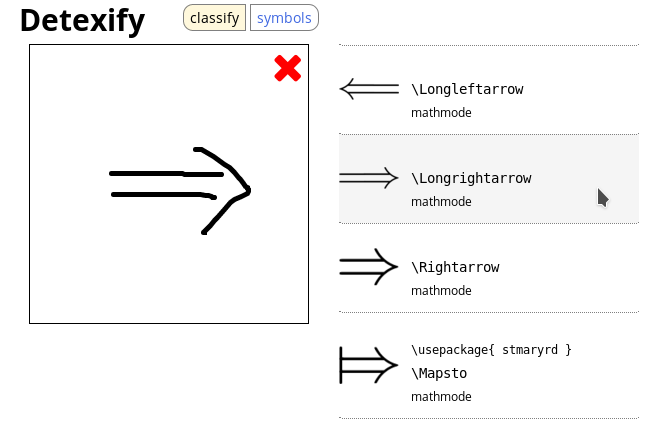
\includegraphics[width=\textwidth]{img/detex}~\\~
  Ti permette di disegnare il simbolo e ti mostra il comando per inserirlo, l'ambiente (testo o matematico) ed eventuali pacchetti da importare.


